\chapter{Požiadavky a návrh}

V tejto kapitole zhrnieme požiadavky na aplikáciu a opíšeme jej návrh. V návrhu opíšeme internú štruktúru aplikácie a na vyššej úrovni opíšeme kontrolu ekvivalentných úprav.

\section{Požiadavky}

Požiadavky vyplývajú z toho, že celkovým cieľom aplikácie je kontrola ekvivalentných úprav.
Prvou požiadavkou aplikácie je, že používateľ musí byť schopný pridávať osobitné formuly. Aplikácia musí byť schopná kontrolovať či formuly sú syntakticky správne, prípadne oznámiť používateľovi ak urobil chybu. Aby bola možná kontrola syntaxu formuly aplikácia potrebuje poznať prvorádový jazyk, v ktorom sú formuly napísané. Preto druhou požiadavkou je aby bolo možné zadať aplikácii mimologické symboly jazyka formúl.

Hlavnou požiadavkou je samotná kontrola úprav. Kontrolovanie viacerých rôznych úprav by mohlo viesť k tomu že študent nepochopí úplne tomu čo robí, preto aplikácia bude kontrolovať iba jeden typ úpravy v jednom kroku. Používateľ vyberie akú úpravu má pre dva dané formuly kontrolovať. Počas vývoja sa ale ukázalo, že aby bol kontrolór pohodlnejší na používanie je potrebné kontrolovať aj sofistikovanejšie úpravy, ako je napríklad viacnásobná asociativita a komutativita. Hlavné použitie aplikácie je pre kontrolu prevodu formuly do CNF tvaru. Aplikácia by preto mala pracovať s postupnosťami ekvivalentných úprav a mala byť schopná pracovať s viacerými postupnosťami.

Aplikácia je určená pre výučbu predmetu Logika pre informatikov, kde sa používa elektronický pracovný zošit, výrobený ako súčasť inej bakalárksej práce \cite{logicworkbook}. Väčšina úloh pre študentov predmetu je zadávaná a riešená v elektronickom zošite, preto požiadavkou je, že aplikácia by mala byť do neho integrovaná. Táto požiadavka znamená, že používateľské rozhranie bude vyrobené pomocou knižnice React a tiež že bude možné stav aplikácie ľahko uložiť a načítať.


\section{Návrh}

\subsection{Návrh stavu aplikácie}\label{navrhstavu}

Stav aplikácie bude rozdelený na 3 časti: jazyk, úpravy a ukladanie/načítanie. Každá časť bude uchovávať iba nevyhnutné dáta. V stave nebude potrebné ukladať komplexnejšie dáta, ktoré vieme odvodiť z uložených.

Prvá časť stavu bude určená pre logický jazyk, konkrétne pre mimologické symboly. Jazyková časť si bude pamätať text vložený do textových polí pre konštanty, predikáty a funkcie. Všetky formuly využívajú logický jazyk pri premene do stromových reprezentácií. Kvôli efektívnosti je ideálne vyhnúť sa použitiu chybným vstupom mimologických symbolov, preto si jazyková časť bude tiež pamätať posledné validné vstupy pre texty, ktoré sa použijú pri kontrolovaní formúl.

Druhá časť stavu bude pre samotné formuly a úpravy. Časť si bude pre každú formulu pamätať jej jedinečné identifikačné číslo, text z textového polia, zvolenú ekvivalentnú úpravu a číslo predošlej formuly (číslo formuly, na ktorú sa úprava aplikovala). Keďže hlavným účelom aplikácie je prevod formuly do CNF tvaru postupným aplikovaním ekvivalentných úprav, v stave budú tiež zapamätané postupnosti identifikačných čísel formúl a tiež identifikačné číslo danej postupnosti.  Pre podporu skolemizácie bude v tejto časti vstupy textových polí pre skolémove konštanty a funkcie a identifikačné číslo formuly, pri ktorej vznikli.

Posledná časť bude určená pre ukladanie a načítanie stavu. Jediné čo bude v tejto časti zapísané je chybová hláška ak načítanie stavu zlyhá.



\subsection{Návrh kontroly úprav}

\begin{figure}[tbh]
\centerline{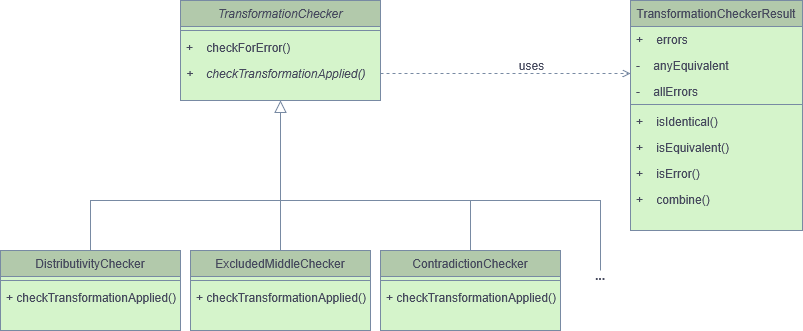
\includegraphics[width=\textwidth]{images/BcMatchingClassDiagram}}
\caption[Diagram tried kontroly úprav]{Diagram tried kontroly ekvivalentných úprav}
\label{obr:ClassDiagram}
\end{figure}

Hlavný problém pri kontrole ekvivalentných úprav je, že úprava mohla nastať ľubovoľný počet krát v ľubovoľnej časti formuly. Ak by sme kontrolovali každé miesto kde by mohla nastať úprava, riešenie by bolo príliš neefektívne a pomalé. Ale môžeme využiť to, že jedna formula vznikla úpravou druhej formuly, a preto buď je časť prvej formuly rovnaká s časťou druhej formuly, alebo nastala úprava. Ak pri súčasnom rekurzívnom prechádzaní stromových reprezentácií obidvoch formúl nájdeme rozdiel, môžeme usúdiť že sa používateľ na danom mieste pokúsil urobiť ekvivalentnú úpravu. Problém nastane, keď niektoré ekvivalentné úpravy nemenia časti formúl, ako napríklad úpravy \eqref{upravy:8}, kde obidve formuly zdieľajú tú istú spojku. Týmto spôsobom by sme preskočili rovnakú spojku a našli rozdielne neekvivalentné podformuly, z toho by sme zle usúdili, že nastala chyba. Toto vyriešime tým, že chyby budú \uv{prebublávať} hore. Ak sa program rekurzívne dostal do koreňa $A$ a našiel chybu v jeho podstrome tak sa pozrie, či nenastala úprava v koreni $A$. Riešenie sa síce spomalí, ale vďaka tomu že kontrolór je určený ako učebná pomôcka, stromové reprezentácie vstupných formúl nebudú príliš hlboké, a preto spomalenie je zanedbateľné.

Výsledok kontroly bude reprezentovaný osobitnou triedou. Trieda výsledku bude obsahovať metódy na zistenie výsledku a tiež metódu na kombinovanie výsledkov. Možné hodnoty výsledku budú tri: identický, ekvivalentný a chybný. Identický výsledok znamená, že podstromy sú identické. Ekvivalentný výsledok je vrátený, keď v podstrome nastala aspoň jedna ekvivalentná úprava a všetky úpravy sú bezchybné. Chybný výsledok znamená, že v podstrome nastala buď chybná úprava, alebo iná chyba. Navyše obsahuje chybnú hlášku, ktorá sa neskôr zobrazí používateľovi. 

\label{checkeralgorithm}Rôzne ekvivalentné úpravy budeme reprezentovať osobitnými triedami pre každú úpravu. Triedy budú odvodené z abstraktnej triedy, ktorá bude obsahovať spoločnú časť algoritmu kontroly. Triedy sa budú líšiť v časti, ktorá usúdi či na konkrétnom mieste formuly nastala ekvivalentná úprava. Diagram tried je zobrazený v obrázku \eqref{obr:ClassDiagram}. Pseudokód spoločnej rekurzívnej časti kontroly je nasledovný:

\begin{lstlisting}[]
checkForError(orig, trans) {
    if (sameFunctor(orig, trans)) {
        result = checkChildren(orig, trans)
        if (result.isEquivalentOrIdentical()) {
            return result
        }
    }
    return checkTransformationApplied(orig, trans)
}
\end{lstlisting}

Metódy \texttt{sameFunctor} a \texttt{checkChildren} budú súčasťou abstraktnej triedy. Funkcia \texttt{sameFunctor} zistí či korene stromov sú rovnaké (či sú obidva korene rovnaké spojky, rovnaké quantifikátory s rovnakými premennými atď.). Keďže stromové reprezentácie formúl sú n-árne metóda \texttt{checkChildren} zavolá rekurzívnu kontrolu koreňov všetkých podstromov a skombinuje ich výsledky. Metóda \texttt{checkTransformationApplied} je abstraktná, ktoré konkrétne triedy prepíšu. Ak ekvivalentná úprava nastala, tak bude potrebné zavolať rekurziu na iné podstromy než tie ktoré skontrolovala \texttt{checkChildren}. Z toho dôvodu metóda tiež zavolá rekurzívnu kontrolu všetkých potrebných podstromov.



